\documentclass[]{article}
\usepackage{graphicx}
\graphicspath{ {./images/} }
\usepackage{hyperref}

\hypersetup{
	colorlinks=true,
	linkcolor=blue,     
	urlcolor=blue
}

%opening
\title{CSCI 470 - Note-taking application requirements}
\author{Logan Humbert}

\begin{document}
	
	\maketitle
	
	\pagebreak
	
	\tableofcontents
	
	\listoffigures
	
	\pagebreak
	
	\section{Description of the application}
	
	This little mobile application aims to let students taking notes for their different classes, and organizing them by class.
	
	\section{Requirements}
	
	\begin{itemize}
		\item \textbf{Who are the users? } The users are students (College, High School, Middle School, ...)
		
		\item \textbf{Who are the customers?} This app is only made in a school context. There is no real customer for it.
		
		\item  \textbf{User stories:}
			\begin{itemize}
				\item As a new user, I want to add my different classes, and start adding notes for them
				
				\item  As a regular user, I keep adding a new note during a lecture in my different classes, then I review them when I study.
				I can easily modify the content of the note if I need to.
			\end{itemize}
		
	\end{itemize}
	
	\section{Features}
	
	The user should be able to complete these different tasks easily:
	
	\begin{itemize}
		\item See his different classes
		\item Add/edit or delete a class
		\item Create/edit/delete a note for any class he has created
		\item View a note
		\item  Search for a class or a note by typing a part of its name
	\end{itemize}
	
	\pagebreak
	
	\section{Design}
	
	\subsection{Sketches on paper}
	
	Here is a first sketch of the different pages of the app, and the transitions between them:
	
	\begin{figure}[!htb]
		\centering
		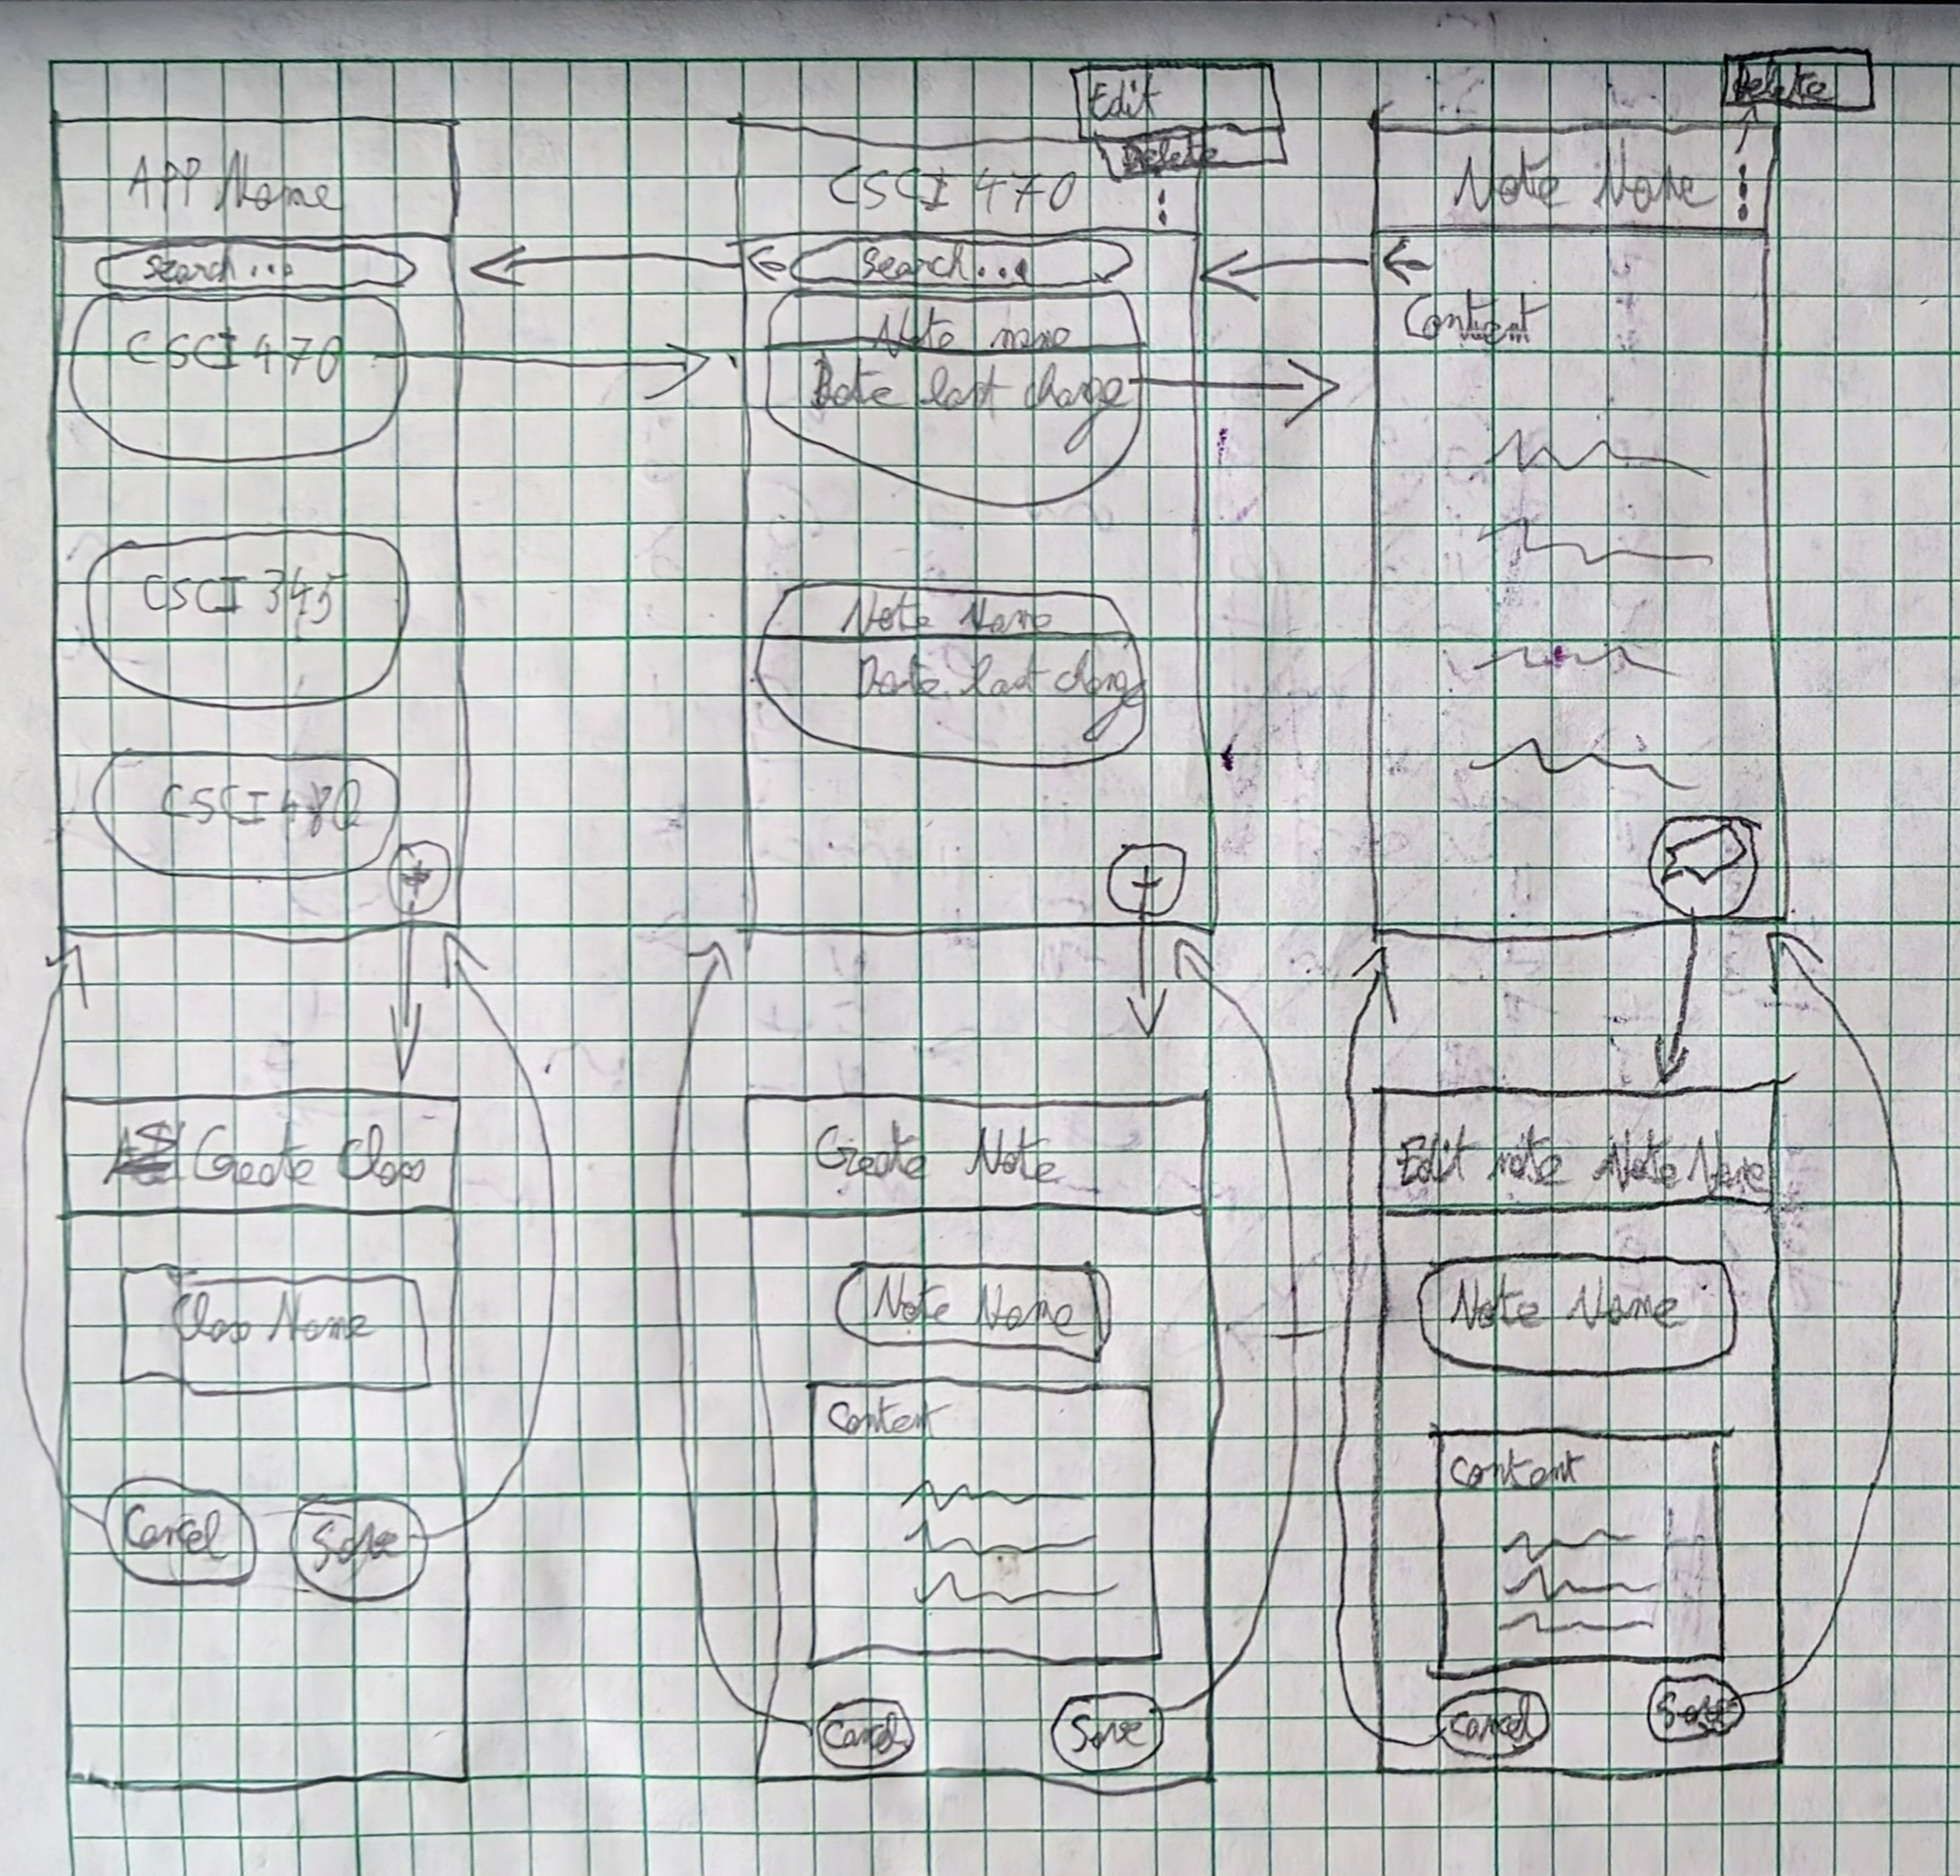
\includegraphics[scale=0.1]{first_sketch}
		\caption{First sketch on paper}
	\end{figure}
	
	I imagine having 5 different screens:
	
	\begin{itemize}
		\item The home page, containing a list of the existing classes.
		\item The add/edit class form
		\item The list of notes in a class
		\item The add/edit note form
		\item The content of a note
	\end{itemize}
	
	All pages can be accessed by clicking on a specific element, as the arrows on the sketches show.
	
	\pagebreak
	
	\subsection{Prototyping on Figma}
	
	After drawing my first sketches on paper, I started making a more accurate and clean design of the UI on Figma, and I used its prototyping features to create the transitions between the pages of the app.
	
	As Flutter uses the Google Material's design, I used their official figma template, which contains reusable Material component, so my Figma design could be as close as possible as the UI the final app will have.
	
	You can access my figma design \href{https://www.figma.com/file/ZOlxVGHb9fLdk5uUODqMU9/CSCI-337---Notes-Taking-App?type=design&node-id=54810%3A34721&mode=design&t=fS6KJvRgsvtgz9cf-1}{here}.
	
	I started by making the User Story "Create a class"
	
		\begin{figure}[!htb]
		\centering
		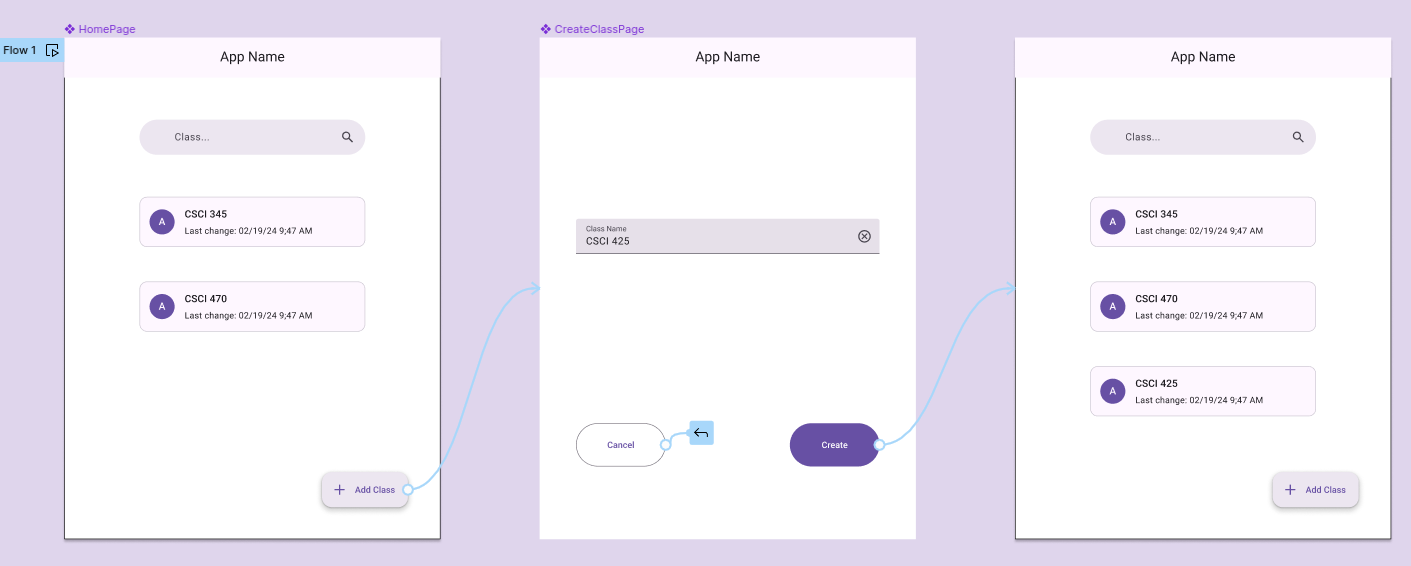
\includegraphics[scale=0.3]{figma_user_story_create_class}
		\caption{User story "Create Class" on Figma}
	\end{figure}
	
	From the home page that contains the list of our classes, a button lets the user create a class by giving it a name. It is then immediately available from the home page.
	
	\pagebreak
	
	Then I added the other user stories and added transitions between the different pages of the app:
	
	\begin{figure}[!htb]
		\centering
		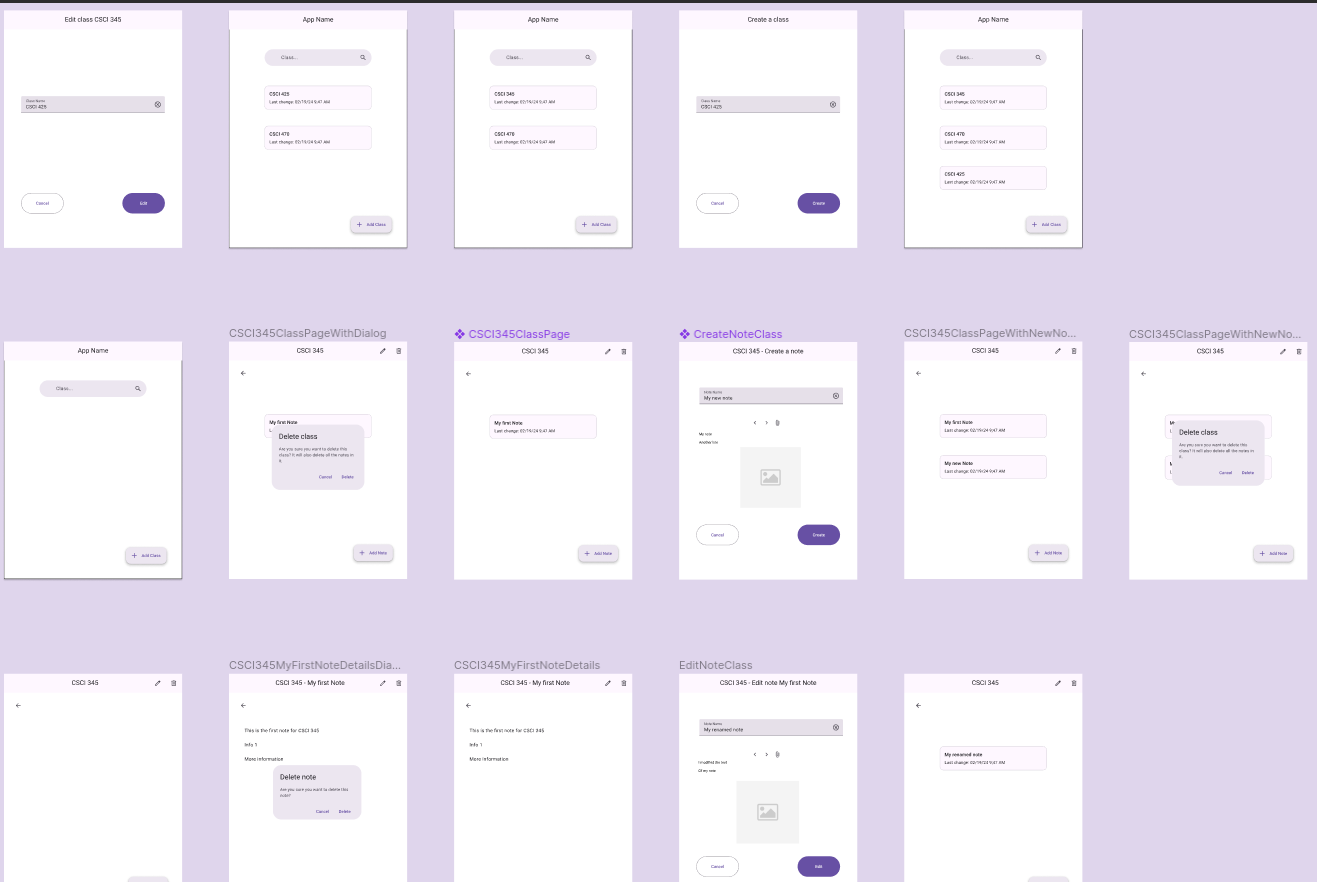
\includegraphics[scale=0.3]{figma_user_stories_finish}
		\caption{All user stories on Figma}
	\end{figure}
	
	Some pages of the app have been duplicated, as they simulate a change in database, or they display an additional graphical element, such as a dialog box.
	These are used to obtain a better experience when we execute the prototype on figma.
	
	\pagebreak
	
	\section{Links}
	
	Here are the links to important resources:
	
	\begin{itemize}
		\item \href{https://github.com/Logan-Developer/ui-lahumbert/tree/main/FinalProject}{Project's repository} 
		
		\item \href{https://www.figma.com/file/ZOlxVGHb9fLdk5uUODqMU9/CSCI-337---Notes-Taking-App?type=design&node-id=54810%3A34721&mode=design&t=fS6KJvRgsvtgz9cf-1}{Figma Design}
	\end{itemize}
	
	\label{LastPage}
\end{document}